\section{Lernen von Superpixeln}

\begin{itemize}
  \item \textbf{SuperCNN:} anstatt eines Bilders wird eine Sequenz von Superpixeln in das CNN gefüttert
  \item \underline{Problem:} kontextbezogene Informationen gehen verloren (Methoden wie Superpixel Lattices adressieren dieses Problem, opfern aber Genauigkeit)
  \item $\Rightarrow$ zwei Kernel sollen Information wiederherstellen:
  \begin{enumerate}
    \item \emph{Spatial Kernel:} beschreibt Einzigartigkeit der Farben
    \item \emph{Range Kernel:} beschreibt Farbverteilung
  \end{enumerate}
  \item \underline{zusätzlich:} Multiscale Strukur des Netzes mit \emph{Shared Weights}
\end{itemize}

\begin{figure}[h]
  \centering
  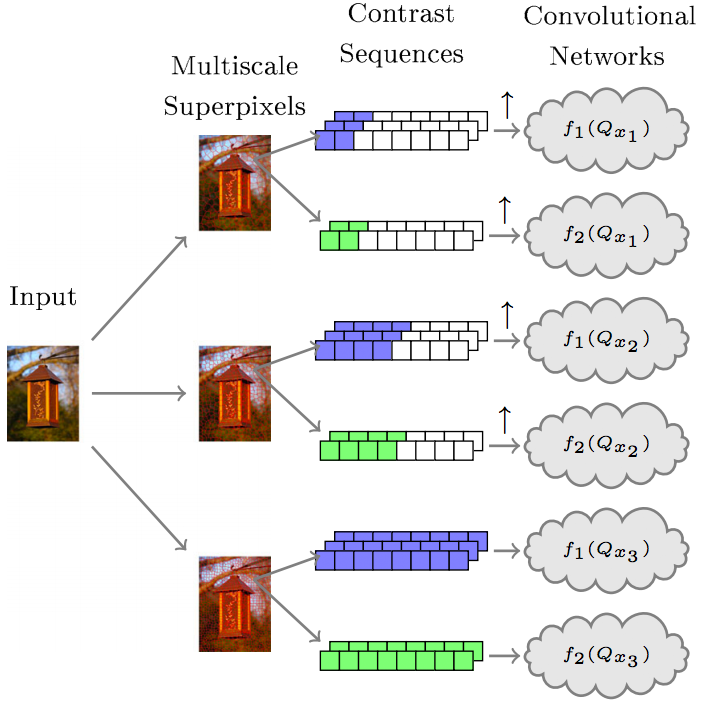
\includegraphics[width=.8\textwidth]{images/superpixel_learning}
\end{figure}

\begin{itemize}
  \item SuperCNN berechnet für individuelles Bild in etwa genauso lange wie klassische CNNs auf Bildern (~0.45s)
  \item \underline{Vorteile:}
  \begin{itemize}
    \item benötigt weniger Trainingsdaten
    \item Trainingsdaten werden generalisierter genutzt $\Rightarrow$ Netz fällt es leichter, für unbekannte Bilder Gemeinsamkeiten zu erkennen
    \item gleiche oder bessere Performance
  \end{itemize}
\end{itemize}
